\pagestyle{fancy}
\chapter{Query processing}
\label{chap:Query processing}
\pagestyle{fancy}

Query processing in a vector database is the process of searching for the most relevant results from a collection of vectors. It starts with a search specification, which includes a similarity score and the type of query; all of these are provided by users through a query interface.
After receiving the query, the system processes it by running a series of steps in the vector collection. These steps include simple similarity searches and faster methods that use indexes to improve efficiency. This ensures that the search is handled quickly and returns accurate results.
\section{Vector similarity search}
The goal of a vector similarity search is to efficiently identify vectors that are most similar to a given query vector based on a specified distance or similarity metric. This search process is often used in high-dimensional spaces, where traditional search techniques can become computationally expensive. Several types of vector similarity search techniques exist, each with its trade-offs in terms of accuracy, efficiency, and applicability to different problems.
\subsection{Distance metrics}
Vector similarity search leverages the mathematical properties of vectors to find the most relevant vectors in a database in response to a query. This is done by evaluating the distance metric between the query vector \textbf{q} and the vectors \textbf{v} in the database. A distance score, often denoted \textbf{d(q,v)}, calculates a scalar value of the two \textbf{D}-dimensional vectors, where a smaller value indicates greater similarity between the vectors. The vectors with the lowest distance scores are considered the most similar to the query vector.

\begin{itemize}
    \item \textbf{Euclidean Distance:} Measures the straight-line distance between two points in a D-dimensional space.
    \[
    d(a, b) = \sqrt{\sum_{i=1}^{D} (a_i - b_i)^2}
    \]
    \item \textbf{Manhattan Distance (L1 Norm):} Calculates the sum of absolute differences between the coordinates of two vectors.
    \[
    d(a, b) = \sum_{i=1}^{D} |a_i - b_i|
    \]
    \item \textbf{Cosine Similarity:} Computes the cosine of the angle between two vectors, often used as a similarity metric. The corresponding distance is:
    \[
    d(a, b) = 1 - \frac{\sum_{i=1}^{D} a_i b_i}{\sqrt{\sum_{i=1}^{D} a_i^2} \sqrt{\sum_{i=1}^{D} b_i^2}}
    \]
    \item \textbf{Jaccard Distance:} Used for binary or sparse data, defined as:
    \[
    d(a, b) = 1 - \frac{|a \cap b|}{|a \cup b|}
    \]
    \item \textbf{Hamming Distance:} Calculates the number of positions where two binary vectors differ.
    \[
    d(a, b) = \sum_{i=1}^{D} \mathbb{I}(a_i \neq b_i)
    \]
\end{itemize}
\subsection{KNN}
The K Nearest Neighbor algorithm is the most straightforward approach when it comes to Vector Similarity Search, providing an exact result by confronting the k nearest vectors in the vector space. Although this brute-force algorithm provides perfect recall, it requires a lot of computation resources, and, by consequence, the query runtime increases along as the number of data points increases. 
\subsection{ANN}
The Approximate Nearest Neighbor (ANN) algorithm was developed to address the limitations of the k nearest neighbors (kNN) approach, particularly its inefficiency when scaling to large datasets. The primary goal of ANN is to provide near-optimal results while significantly reducing computation time compared to exact kNN searches. Using techniques that approximate nearest neighbors, ANN enables the handling of massive collections of vectors, offering a practical solution for high-dimensional search tasks. The ANN approach also makes use of the vector indexes such as NSW and HNSW that are based on the concept of "six degrees of separation" allowing the algorithm to explore the vector space more efficiently.

\section{Performance metrics}
Assessing the quality of the vector similarity search requires the definition of clear and relevant performance metrics. These metrics provide a standardized way to measure how effectively the search algorithm retrieves the most relevant results from the vector collection, and allows one to find which approach is more suitable for a specific use case.
\begin{itemize}
    \item \textbf{Precision:} Measures the proportion of relevant results among the retrieved results.
    \[
    \text{Precision} = \frac{\text{Number of Relevant Results Retrieved}}{\text{Total Number of Results Retrieved}}
    \]

    \item \textbf{Recall:} Measures the proportion of relevant results that were successfully retrieved.
    \[
    \text{Recall} = \frac{\text{Number of Relevant Results Retrieved}}{\text{Total Number of Relevant Results in the Database}}
    \]
    \item \textbf{Queries Per Second (QPS):} Measures the system's throughput by calculating the number of queries processed per second.
    \[
    \text{QPS} = \frac{\text{Number of Queries Processed}}{\text{Total Time (in seconds)}}
    \]
\end{itemize}


\section{Filtering Techniques}
Filtering techniques in vector search help refine results based on predefined criteria. These techniques ensure that retrieved documents meet specific conditions, improving relevance and accuracy.

\subsection{Pre-filtering}
Pre-filtering applies constraints before executing the search query. This method reduces the search space, leading to faster retrieval times. Common pre-filtering techniques include:
\begin{itemize}
    \item Applying metadata filters (e.g., date, category, author).
    \item Restricting searches to specific document subsets.
    \item Leveraging user-defined conditions for search optimization.
\end{itemize}
\begin{figure}[h]
    \centering
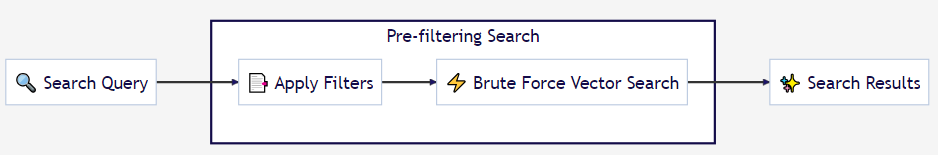
\includegraphics[width=0.8\textwidth]{IMAGES/immagine_2025-03-03_093943770.png}
    \caption{Pre-filtering process. Source: Weaviate\footnotemark[1]}
    \label{fig:Rectangle Tree}
\end{figure}
\footnotetext[1]{\url{https://weaviate.io/blog/speed-up-filtered-vector-search}}
\subsection{Post-filtering}
Post-filtering applies constraints after the search query has been executed. This approach ensures that filtering does not interfere with similarity computations. Common post-filtering techniques include:
\begin{itemize}
    \item Removing results that do not meet certain thresholds.
    \item Applying additional business logic to refine search outputs.
    \item Filtering based on dynamic user preferences after initial retrieval.
\end{itemize}
\begin{figure}[h]
    \centering
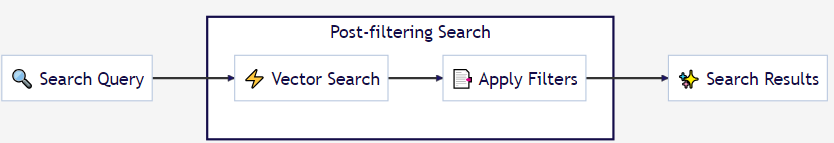
\includegraphics[width=0.8\textwidth]{IMAGES/immagine_2025-03-03_094158324.png}
    \caption{Post-filtering process. Source: Weaviate\footnotemark[1]}
    \label{fig:Rectangle Tree}
\end{figure}
\subsection{In-filtering}
In-filtering integrates filtering conditions directly into the similarity computation process. This technique ensures that relevance scoring inherently considers filtering constraints. Key aspects of in-filtering include:
\begin{itemize}
    \item Modifying similarity calculations to account for filtering parameters.
    \item Embedding constraints within vector representations.
    \item Ensuring efficient and scalable implementation in high-dimensional spaces.
\end{itemize}

\section{ACORN}
ACORN is a predicate-agnostic hybrid search method that extends HNSW to efficiently handle structured query filters. Unlike traditional pre-filtering and post-filtering methods, ACORN achieves sublinear retrieval times even with high-cardinality predicate sets. It constructs a denser graph index and applies predicate-aware traversal strategies to optimize search performance. By leveraging efficient predicate-subgraph traversal while maintaining the speed advantages of HNSW, ACORN provides a scalable and high-performance alternative to traditional hybrid search strategies.

Key parameters governing ACORN's behavior include:
\begin{itemize}
    \item $\gamma$: Neighbor expansion factor.
    \item $M_{\beta}$: Compression parameter for neighbor pruning.
    \item $M$: Degree bound for traversed nodes.
    \item $e$: Fixed entry point to the index.
    \item $s_{min}$: Minimum predicate selectivity.
\end{itemize}

\subsection{Index Construction}
The ACORN-$\gamma$ index is built using two key modifications to HNSW:
\begin{enumerate}
    \item \textbf{Neighbor List Expansion:} Each node collects $M \cdot \gamma$ approximate nearest neighbors instead of the standard $M$. This ensures that filtering operations during search do not fragment the graph.
    \item \textbf{Predicate-Agnostic Pruning:} To counter increased index size, a compression heuristic is applied to bottom-level neighbor lists, reducing memory overhead while maintaining navigability.
\end{enumerate}
A recommended choice for $\gamma$ is $1/s_{min}$, ensuring efficient pre-filtering when selectivity drops below $s_{min}$. This enables ACORN to balance indexing cost and search efficiency.

\subsection{Search Algorithm}
ACORN employs a hierarchical greedy search similar to HNSW but integrates predicate filtering:
\begin{enumerate}
    \item Search begins at the highest level with a fixed entry point ($e$).
    \item Nodes are evaluated based on both distance and predicate constraints.
    \item At each level, the algorithm retrieves filtered neighbors ($N^l_p(v)$), either by:
          \begin{itemize}
              \item Applying a simple predicate filter (truncating to $M$ neighbors).
              \item Expanding two-hop neighbors for enhanced connectivity.
          \end{itemize}
    \item The search proceeds hierarchically until reaching the base level, returning the nearest neighbors that satisfy the query.
\end{enumerate}

\subsection{Complexity Analysis}
\begin{itemize}
    \item \textbf{Index Construction:} $O(n \cdot \gamma \cdot \log(n) \cdot \log(\gamma))$, where $n$ is the dataset size.
    \item \textbf{Search Complexity:} $O((d + \gamma) \cdot \log(s \cdot n) + \log(1/s))$, closely approximating HNSW’s complexity with minor overhead.
\end{itemize}


\subsection{Weaviate's Implementation of ACORN}
Weaviate modifies ACORN with:
\begin{itemize}
    \item 	\textbf{Graph Construction:} Retains HNSW’s original pruning logic to reduce resource overhead and support seamless activation without reindexing.
    \item 	\textbf{Graph Exploration:} Uses two-hop expansion only when the first-hop node fails the filter, optimizing performance in high-filter-density regions.
    \item 	\textbf{Entry Point Seeding:} Introduces additional entry points at layer zero to improve retrieval efficiency in low-filter-density areas.
    \end{itemize}
\subsection{Performance Analysis on Weaviate}
In the following figures, we present a performance comparison of different filtering strategies. The first figure compares pre-filtering and post-filtering, where post-filtering has been expanded to account for filter selectivity. While its recall improves and approaches that of pre-filtering, this comes at the cost of higher resource usage. 
The second figure compares the default and ACORN filtering strategies, showing that ACORN achieves slightly better performance with lower resource usage. The study was conducted on the TripClick vector dataset (800k vectors of 768 dimensions) using an HNSW index.

\
\begin{figure}[h]
    \centering
    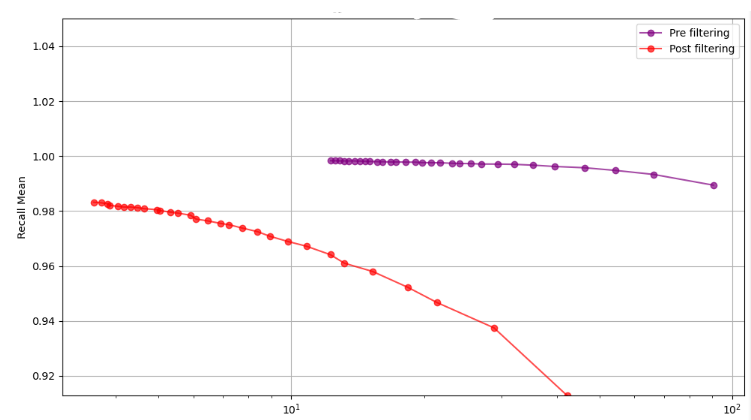
\includegraphics[width=0.4\textwidth]{IMAGES/immagine_2025-03-03_154956860.png}
    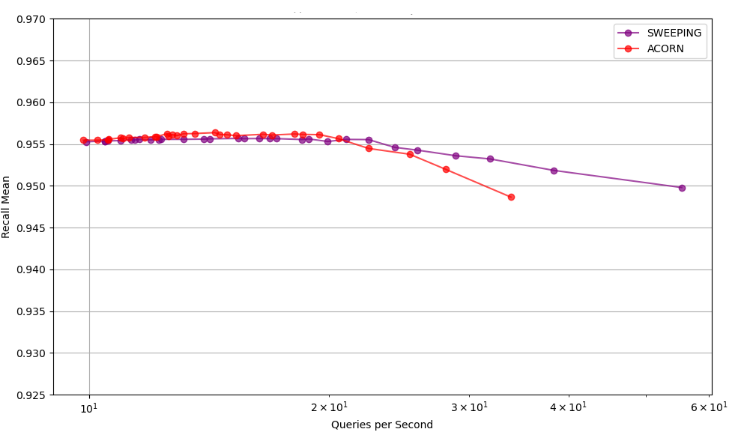
\includegraphics[width=0.4\textwidth]{IMAGES/immagine_2025-03-03_150720257.png}
    \caption{Performance comparison in Weaviate.}
    \label{fig:Weaviate}
\end{figure}
\section{Range Filtering ANN}
Range Filtering ANN (RFANN) is used for high-dimensional data where each vector has an associated, ordered attribute. Given a dataset \( D \), a query vector \( q \), a parameter \( K \), and a query range \([x, y]\), RFANN aims to find the approximate \( K \) nearest upper neighbors in \( D \) whose attributes fall within \([x, y]\). This is valuable in applications like e-commerce, where users filter products by price. However, such searches can be computationally expensive. Common approaches—Post-Filtering, In-Filtering, and Pre-Filtering—each have limitations: Post- and In-Filtering struggle with high-selectivity queries, while Pre-Filtering becomes inefficient with large datasets. Optimizing resource usage and performance remains a key challenge.


\section{Naive Solution}
A simple but impractical approach to solving range-filtering approximate nearest neighbor (RFANN) queries is to build dedicated graph-based indexes for all possible query ranges. However, this does not scale well. Given a collection of $n$ objects, the number of possible query ranges grows to $O(n^2)$. 

\section{IRangeFiltering}
IRangeGraph is a novel method designed to handle range-filtering queries efficiently without constructing a massive number of dedicated indexes. Instead of materializing a separate graph for each query range, \textbf{IRangeGraph constructs a moderate number of precomputed graphs, called elemental graphs}, which are later used to dynamically build the required index for any given query range.

The key benefits of IRangeGraph are:
\begin{itemize}
    \item \textbf{On-the-fly graph construction}: Instead of storing all possible dedicated graphs, it dynamically assembles a graph from \textit{elemental graphs} corresponding to segments of the data.
    \item \textbf{Efficient querying}: Despite constructing the graph during query execution, the overhead is low, and performance is close to that of fully materialized dedicated graphs, while using significantly less memory.
\end{itemize}

\subsection{Constructing Elemental Graphs and Forming Dedicated Graphs}
To efficiently construct elemental graphs, \textbf{IRangeGraph leverages a segment tree}:
\begin{itemize}
    \item The segment tree has \textbf{$O(\log n)$ layers}, where each node represents a range of objects.
    \item The \textbf{root node} corresponds to the entire dataset.
    \item Each \textbf{child node} represents a sub-range, recursively partitioning the dataset into smaller segments.
    \item \textbf{Leaf nodes} correspond to individual objects (segments of size 1), meaning it contains elements with the same values.
    \item Each segment stores an \textbf{elemental graph}, which serves as a building block for constructing query-specific graphs \cite{irangegraph}.
\end{itemize}


Each \textbf{node} in the segment tree, not just the leaves, has its own elemental graph materialized. This means that an elemental graph is constructed for every segment at every level of the segment tree, leading to a total of $O(n \log n)$ elemental graphs across the entire structure \cite{irangegraph}.



\subsection{Dedicated Graph Construction}
In order to construct on-the-fly the dedicated graph, IRangeGraph utilizes the concept of the \textbf{Relative Neighborhood Graph (RNG)}. Which ensures that an edge between two objects exists only if no other object is significantly closer to both of them. This pruning rule helps maintain a sparse yet effective structure for nearest neighbor search. 

When a query is issued with a given range $[L, R]$, IRangeGraph constructs the required graph dynamically:
\begin{enumerate}
    \item Identify the \textbf{elemental graphs} that intersect with the query range.
    \item Combine relevant edges from these elemental graphs to form the dedicated graph.
    \item Apply \textbf{RNG pruning rules} to retain only essential edges.
\end{enumerate}


\subsubsection{Example: Querying a Specific Range}
Consider a dataset with values in the range $[0,4]$ and an issued query for the range $[2,3]$. The segment tree structure would include:
\begin{itemize}
    \item A root node covering the full range $[0,4]$.
    \item Child nodes covering $[0,2]$ and $[3,4]$.
    \item Further subdivisions where necessary, with leaf nodes at individual values.
\end{itemize}

\begin{figure}[h]
    \centering
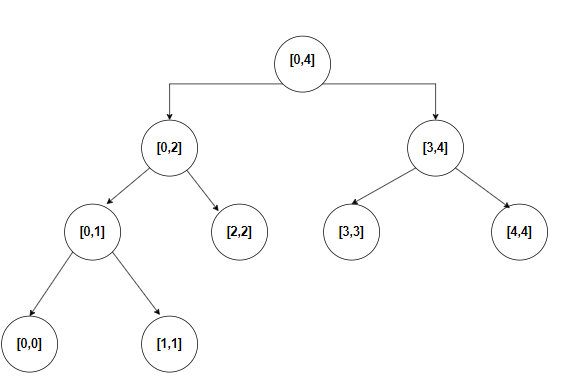
\includegraphics[width=0.8\textwidth]{IMAGES/immagine_2025-02-28_120223507.png}
    \caption{Example of Segment Tree.}
    \label{fig:Segment Tree}
\end{figure}

For the query $[2,3]$:
\begin{enumerate}
    \item The elemental graphs corresponding to segments $[2,2]$ and $[3,3]$ are selected since they fully intersect with the query range.
    \item Additionally, the segment $[2,3]$ is selected, as it directly encompasses the range.
    \item The relevant edges from these elemental graphs are combined to construct the dedicated graph.
    \item The resulting graph enables efficient nearest neighbor search within the range $[2,3]$.
\end{enumerate}

\section{Segment Graph for RFANN Search (SeRF)}
SeRF addresses the issue of the Naive approach by introducing a \textit{segment graph}, which losslessly compresses these $n$ HNSW indexes into a single structure with a significantly reduced memory footprint. The data structure is refereed as Segment Graph, which organizes the neighbor relationships dynamically across different ranges, permitting to represent the the connectivity of $n$ HNSW graphs using only $\mathcal{O}(nM)$ space, where $M$ is the maximum degree of nodes in HNSW.

This is achieved through:
\begin{itemize}
    \item Storing each edge only once, annotated with its active range $[b, e]$, instead of duplicating it across multiple graphs.
    \item Avoiding the explicit storage of $n$ independent HNSW graphs, leading to a compression factor of approximately $\mathcal{O}(n)$ in the worst case.
    \item Ensuring efficient query execution by enabling range-based edge retrievals without reconstructing multiple indexes.
\end{itemize}

\subsection{Segment Graph construction}
The construction follows these key steps:
\begin{enumerate}
    \item \textbf{Sequential HNSW Insertion:}  
    Data points are sorted based on their associated attribute values. The HNSW graph is incrementally built in an ordered manner, meaning that at step $x$, the index constructed so far contains only the first $x$ points.

    \item \textbf{Tracking Persistent Neighbor Relationships:}  
    When adding a new point $v_x$ to the graph, its approximate nearest neighbors are determined using an ANNS search over the existing structure. These neighbors are then pruned to ensure efficient navigation in the HNSW hierarchy. Instead of storing these neighbor connections separately for each step, we record their validity over a \textit{segment range} $[b, e]$, where:
    \begin{itemize}
        \item $b$ represents the insertion step when the edge was first added.
        \item $e$ represents the step at which the edge was removed due to the pruning process.
    \end{itemize}
    
    \item \textbf{Segment-Based Edge Storage:}  
    Each edge $(v_i, v_j)$ in the segment graph is stored as a tuple $(v_j, b, e)$ in the adjacency list of $v_i$. This means that $v_j$ remains a neighbor of $v_i$ in all query-specific graphs from step $b$ to $e$. Instead of storing $n$ redundant graphs, this method encodes all necessary information in a single compressed structure.

    \item \textbf{Edge Pruning and Updates:}  
    When a new node $v_x$ is inserted, it may cause the removal of certain edges due to dominance criteria in HNSW pruning (i.e., when a new node provides a more efficient navigation path). The segment graph updates the validity range of affected edges dynamically, ensuring that removed edges are correctly marked with an endpoint $e = x - 1$.
\end{enumerate}

\section{Further Compression of the Segment Graph}  
SeRF compresses multiple HNSW indexes into a single segment graph but is limited to static datasets. The \textbf{Dynamic Range-Filtering Approximate Nearest Neighbor Search (DRFANN)} model enhances adaptability with a \textit{dynamic segment graph}, enabling incremental updates while reducing redundancy and storage overhead.  

By integrating a rectangle tree and dynamic segment graph, DRFANN surpasses static RFANN methods (SeRF, iRangeGraph, etc.):  
\begin{itemize}  
    \item \textbf{Supports Dynamic Data:} Allows unordered vector insertions.  
    \item \textbf{Compact Indexing:} Reduces $\mathcal{O}(n^2)$ HNSW graphs to $\mathcal{O}(n \log n)$ edges.  
    \item \textbf{Efficient Queries:} Eliminates costly ANN result merging.  
    \item \textbf{Fast Updates:} Only $\mathcal{O}(\log n)$ edges are modified per insertion.  
\end{itemize}  

\subsection{Dynamic Segment Graph and Compression}  
The \textbf{dynamic segment graph} represents RFANN query ranges in a single, continuously updated structure. Instead of duplicating HNSW graphs, it assigns each edge a rectangular validity label $(l, r] \times [b, e)$, indicating the attribute range where the edge remains valid.  

\subsection{Graph Construction}  
As new vectors arrive, the dynamic segment graph is updated as follows:  
\begin{enumerate}  
    \item \textbf{Rectangle Representation:} Each edge $(v_i, v_j)$ is assigned a validity range $(l, r] \times [b, e)$.  
    \item \textbf{Edge Reuse:} Edges are shared across overlapping query ranges, minimizing storage.  
    \item \textbf{Incremental Updates:} New insertions adjust only $\mathcal{O}(\log n)$ edges, preventing index bloat.  
\end{enumerate}  




\subsection{Rectangle Tree for Space Partitioning}  
The \textit{rectangle tree} hierarchically partitions query ranges, optimizing storage and retrieval:  
\begin{itemize}  
    \item Inserting a vector with attribute \textbf{x} initializes a root node covering $(-\infty, x] \times [x, \infty)$.  
    \item Nearest neighbors are retrieved iteratively, with layer $n$ containing $n$ shared neighbors.  
    \item Nodes represent query ranges $(l, r] \times [b, e]$, reducing redundancy.  
    \item Leaf nodes store approximate nearest neighbors (ANNs) for fast lookup.  
    \item Internal nodes partition the search space, ensuring efficient range-filtered searches.  
\end{itemize}  


\subsection{Example of Insertion in Dynamic Segment Graph}
To better understand the how the Dynamic Segment Graph works, we illustrate the process of the insertion of a new vector. Let the existing dataset consist of nine vectors, each with an associated attribute value, and suppose we insert a new vector:
\[
v10 \quad \text{with attribute value } 54.
\]


\begin{table}[h]
    \centering
    \begin{tabular}{c|c|c}
        \hline
        \textbf{Vector} & \textbf{Distance to $v_{10}$} & \textbf{Attribute} \\
        \hline
        $v_1$ & 2  & 28  \\
        $v_2$ & 18 & 36  \\
        $v_3$ & 17 & 68  \\
        $v_4$ & 8  & 37  \\
        $v_5$ & 4  & 43  \\
        $v_6$ & 11 & 56  \\
        $v_7$ & 9  & 57  \\
        $v_8$ & 13 & 66  \\
        $v_9$ & 10 & 35  \\
        \hline
    \end{tabular}
    \caption{Dataset before inserting $v_{10}$.}
\end{table}


\begin{enumerate}  
    \item Identify the $K$ nearest neighbors using the existing segment graph.  
    \item Initialize an R-tree with root $(-\infty, 54] \times [54, \infty)$, representing $v_{10}$'s rectangle.  
    \item Partition the range space iteratively using the $K$ nearest neighbors.  
    \item Update the \textbf{rectangle tree} to incorporate the new attribute ranges.  
    \item Add edges upon reaching the child nodes.  
\end{enumerate} 



\begin{figure}[h]
    \centering
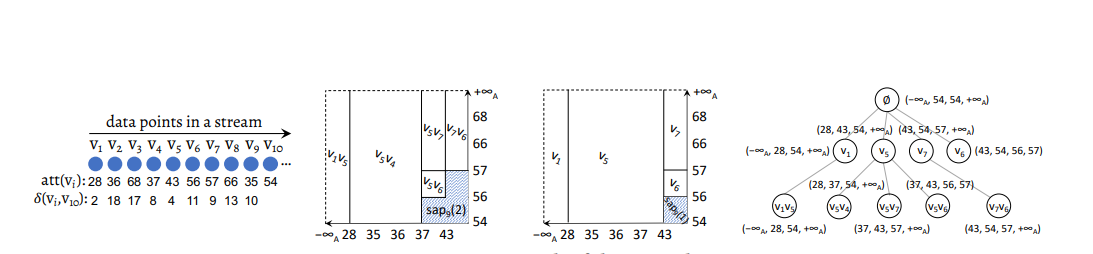
\includegraphics[width=1.1\textwidth]{IMAGES/immagine_2025-03-01_191002770.png}
    \caption{Rectangle Tree and range space partitioning. Source: Miaoqiao\footnotemark[2]}
    \label{fig:Rectangle Tree}
\end{figure}
\footnotetext[2]{\url{https://miaoqiao.github.io/paper/VLDB25_TR.pdf}}